\documentclass[a4paper,12pt]{article}
\usepackage{amssymb} % needed for math
\usepackage{amsmath} % needed for math
\usepackage[utf8]{inputenc} % this is needed for german umlauts
\usepackage[ngerman]{babel} % this is needed for german umlauts
\usepackage[T1]{fontenc}    % this is needed for correct output of umlauts in pdf
\usepackage[margin=2.5cm]{geometry} %layout
\usepackage{booktabs}
\usepackage[hidelinks]{hyperref}
\hypersetup{pdftitle={Balanced Banana},bookmarks=true,}
\usepackage{graphicx}
\usepackage{csquotes}
\usepackage[nonumberlist]{glossaries}
\usepackage{enumitem}
\usepackage{verbatim}
\usepackage{indentfirst} % Adds indent for the first paragraph after a {/section}


\deftranslation[to=ngerman]{Glossary}{\section{Stichwortverzeichnis}}

\makeatletter
\newenvironment{mycode}
 {\def\@xobeysp{\ }\verbatim\rightskip=0pt plus 6em\relax}
 {\endverbatim}
\makeatother

\title{Balanced Banana}
\author{Niklas Lorenz \and Thomas Häuselmann \and Rakan Zeid Al Masri \and Christopher Lukas Homberger \and Jonas Seiler}


%%%%%%%%%%%%%%%%%%%%%%%%%%%%%%%%%%%%%%%%%%%%%%%%%%%%%%%%%%%%%%%%%%%%%%
% Create a shorter version for tables. DO NOT CHANGE               	 %
%%%%%%%%%%%%%%%%%%%%%%%%%%%%%%%%%%%%%%%%%%%%%%%%%%%%%%%%%%%%%%%%%%%%%%
\newcommand\addrow[2]{#1 &#2\\ }

\newcommand\addheading[2]{#1 &#2\\ \hline}
\newcommand\tabularhead{\begin{tabular}{lp{13cm}}
\hline
	}

\newcommand\addmulrow[2]{ \begin{minipage}[t][][t]{2.5cm}#1\end{minipage}%
   &\begin{minipage}[t][][t]{8cm}
    \begin{enumerate} #2   \end{enumerate}
    \end{minipage}\\ }

\newenvironment{usecase}{\tabularhead}
{\hline\end{tabular}}

\usepackage{microtype}

\begin{document}
\pagenumbering{roman}
\begin{titlepage}
    \begin{center}
    
     \vspace*{0.8cm}
 
        
\includegraphics[width=0.5\textwidth]{balancedbanana}
        \vspace*{1cm}
 
        \Huge
        \textbf{Balanced Banana}
 
        \vspace{0.5cm}
        \LARGE
        A Distributed Task Scheduling System
        
        \vspace{0.5 cm}
        \LARGE
        Pflichtenheft
 
        \vspace{1.5cm}

        \large
        \textbf{Niklas Lorenz, Thomas Häuselmann, Rakan Zeid Al Masri, Christopher Lukas Homberger und Jonas Seiler}
 
        \vspace*{0.5cm}

        \textbf{\today}
 
       
        
 
    \end{center}
\end{titlepage}         % Deckblatt.tex laden und einfügen
\setcounter{page}{2}
\tableofcontents          % Inhaltsverzeichnis ausgeben
\clearpage
\pagenumbering{arabic}

\section{Einleitung}
\vspace{0.2cm}
Dieses Dokument dient als Übersicht der Qualitätssicherung. Erläutert werden sowohl unsere Methoden zur Qualitätssicherung als auch das Ergebnis dieser. Ebenfalls beinhaltet dieses Dokument eine Anleitung zum Aufsetzen und Benutzen des endgültigen Programms.
\section{Testabdeckung}
\subsection{Klassenüberdeckung}
\vspace{0.2cm}
Die Testüberdeckung der einzelnen Klassen ist in der ersten Woche der Qualitätssicherung gefallen, dies liegt daran, dass einige Klassen zwar intern funktioneren, sie jedoch im Zusammenspiel mit anderen nicht. In der ersten Woche wurden also hauptsächlich fehlerhafte Schnittstellen oder andere Fehler beseitigt und entsprechende Unit Tests erst in den folgenden Wochen eingeführt. \newline
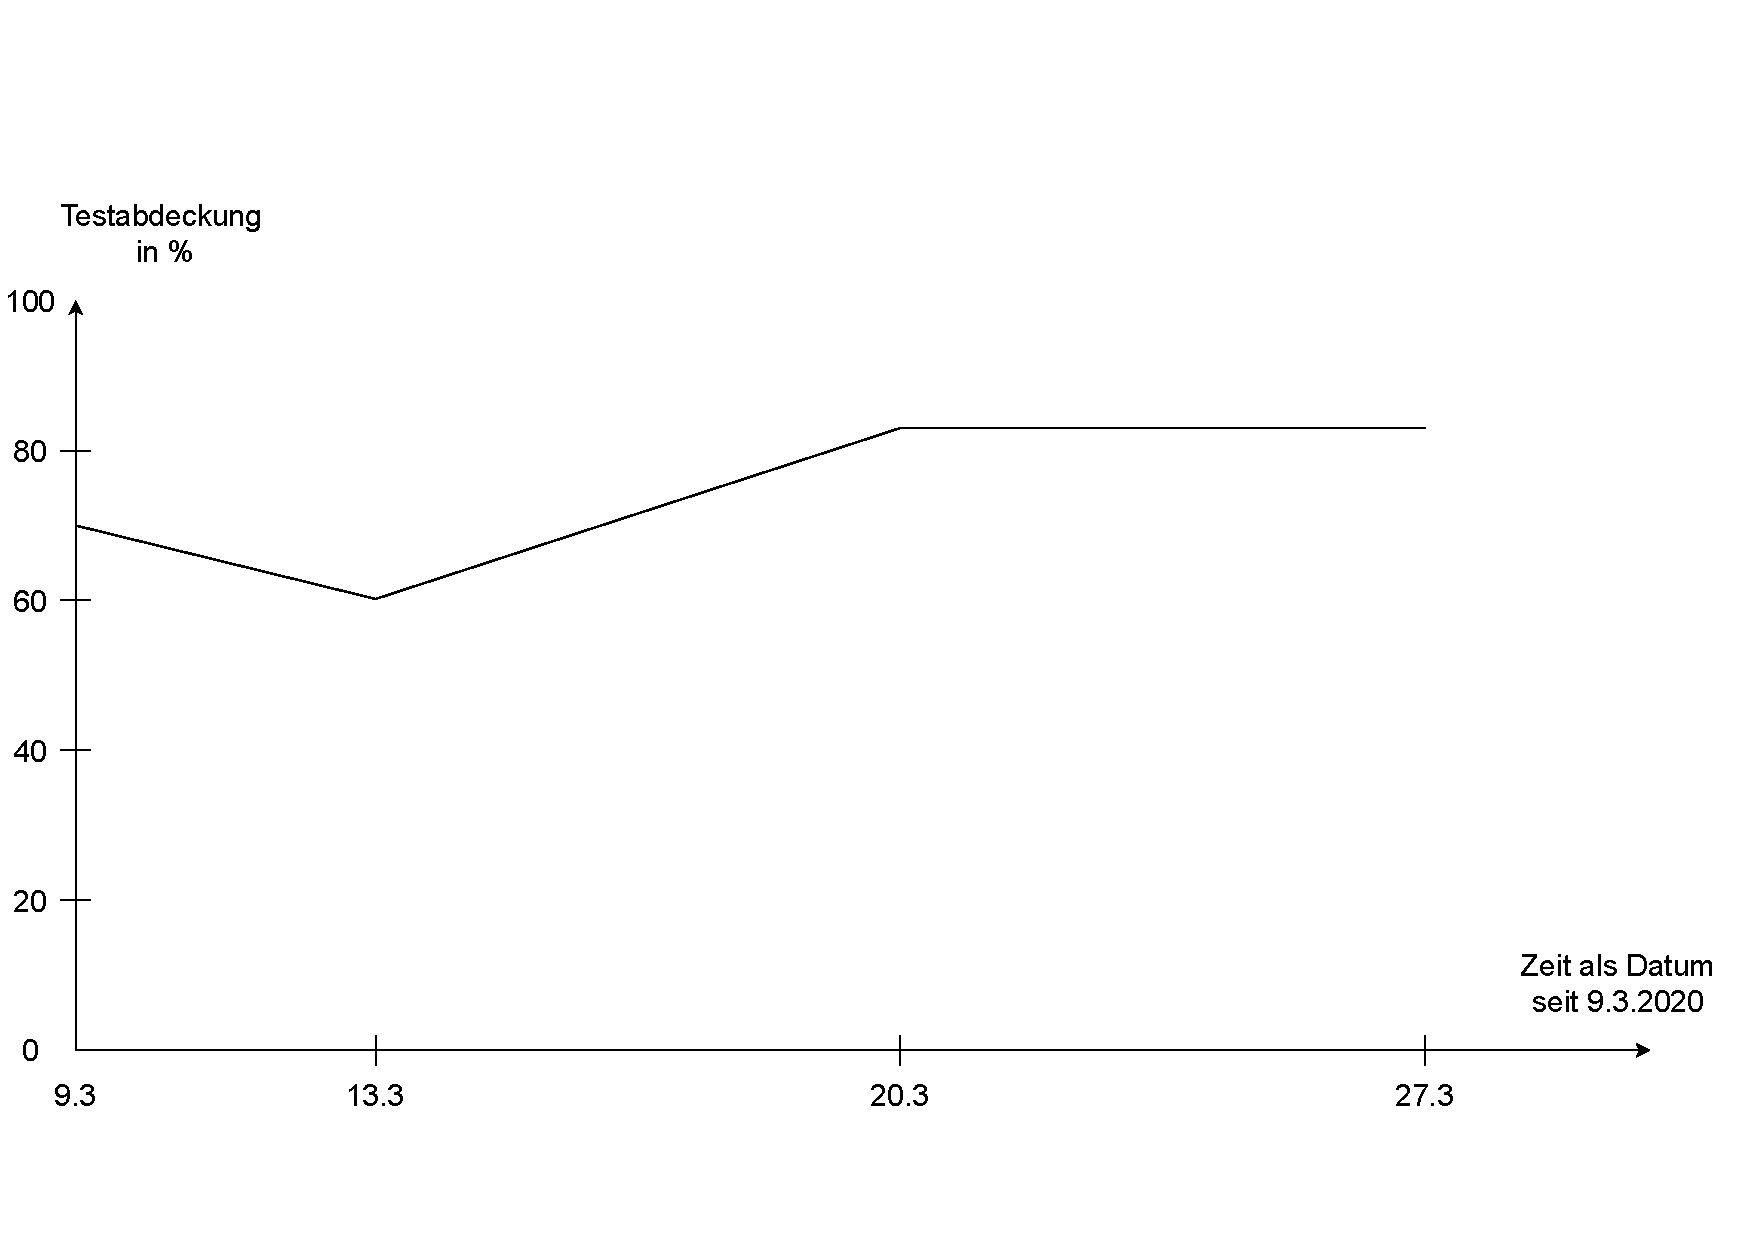
\includegraphics[width=\textwidth]{CoverageD} \newline
Entsprechend sehen wir einen Anstieg in Lines of Code (LOC) sowie der Anzahl Tests.
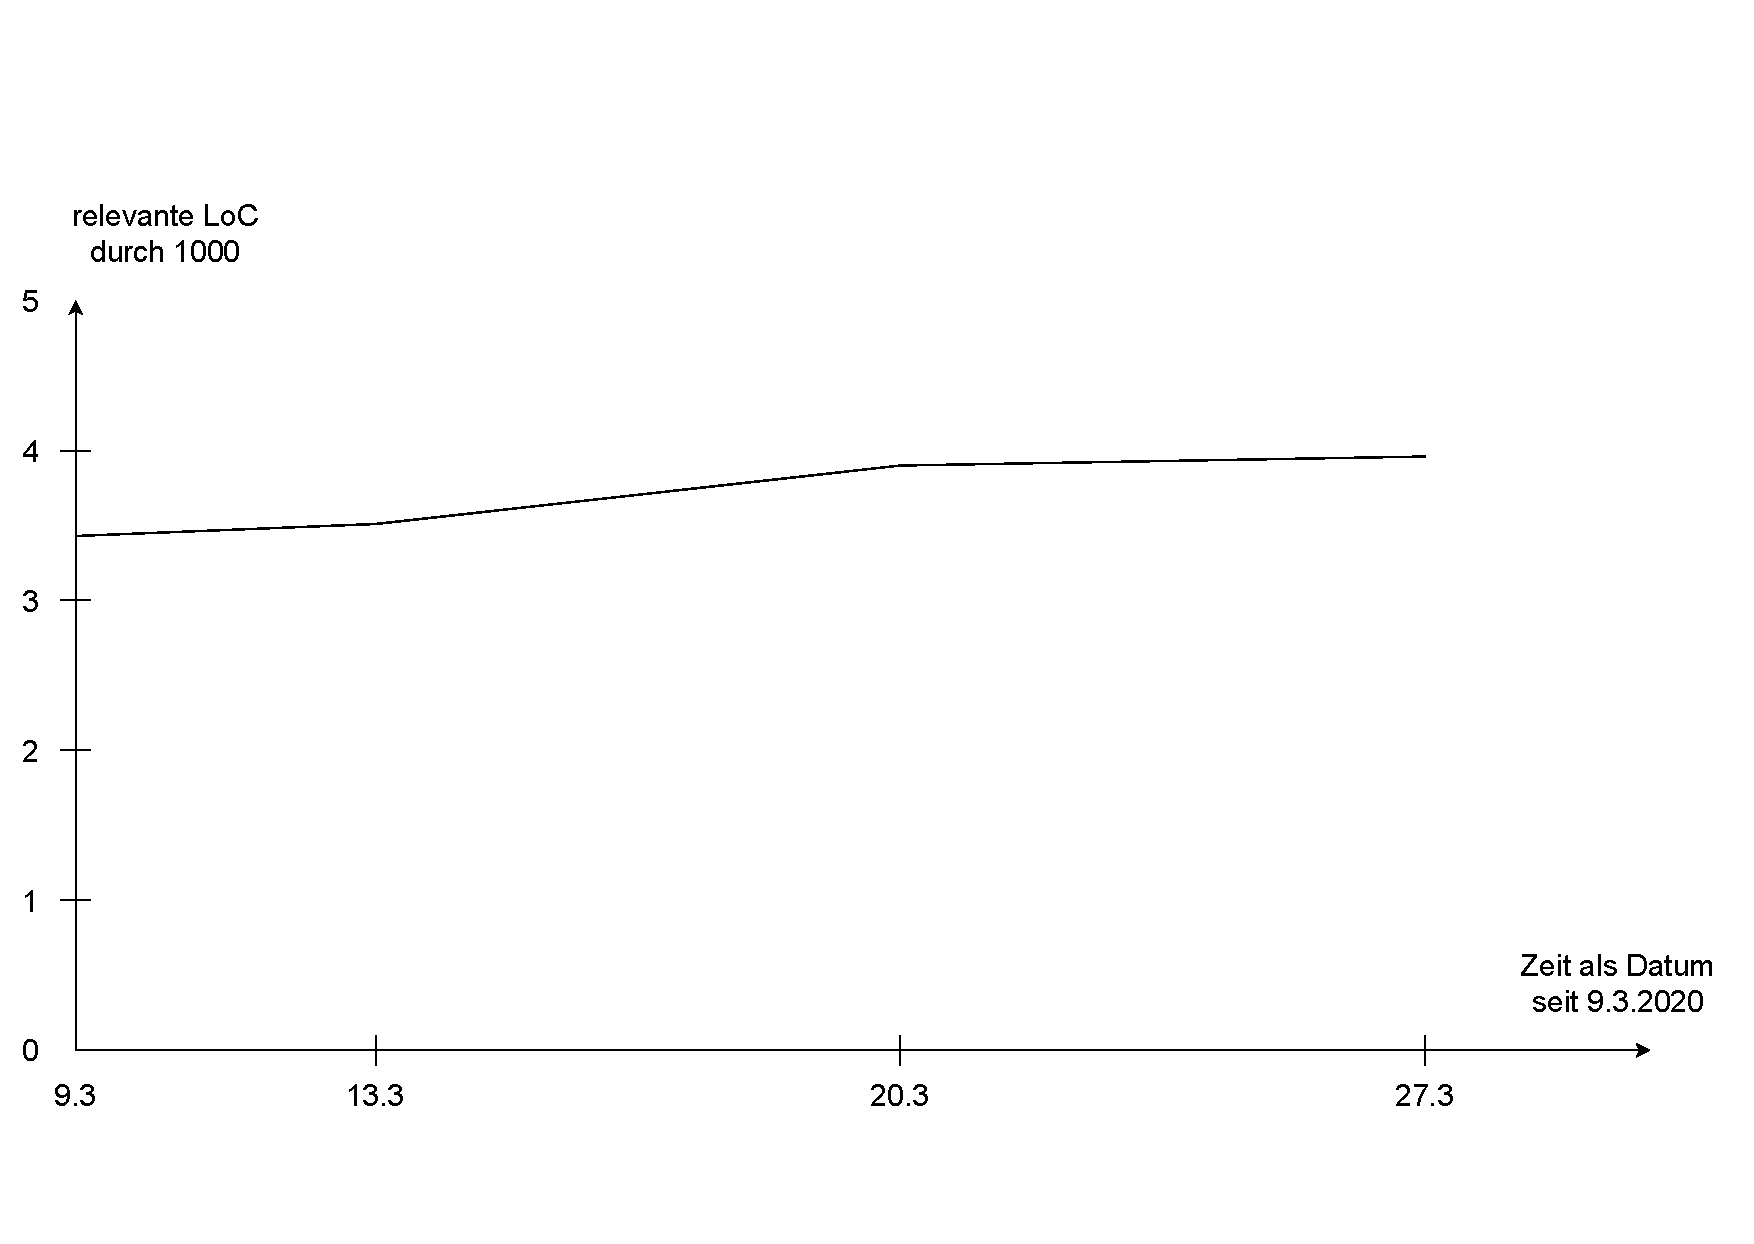
\includegraphics[width=\textwidth]{LOCD} \newline
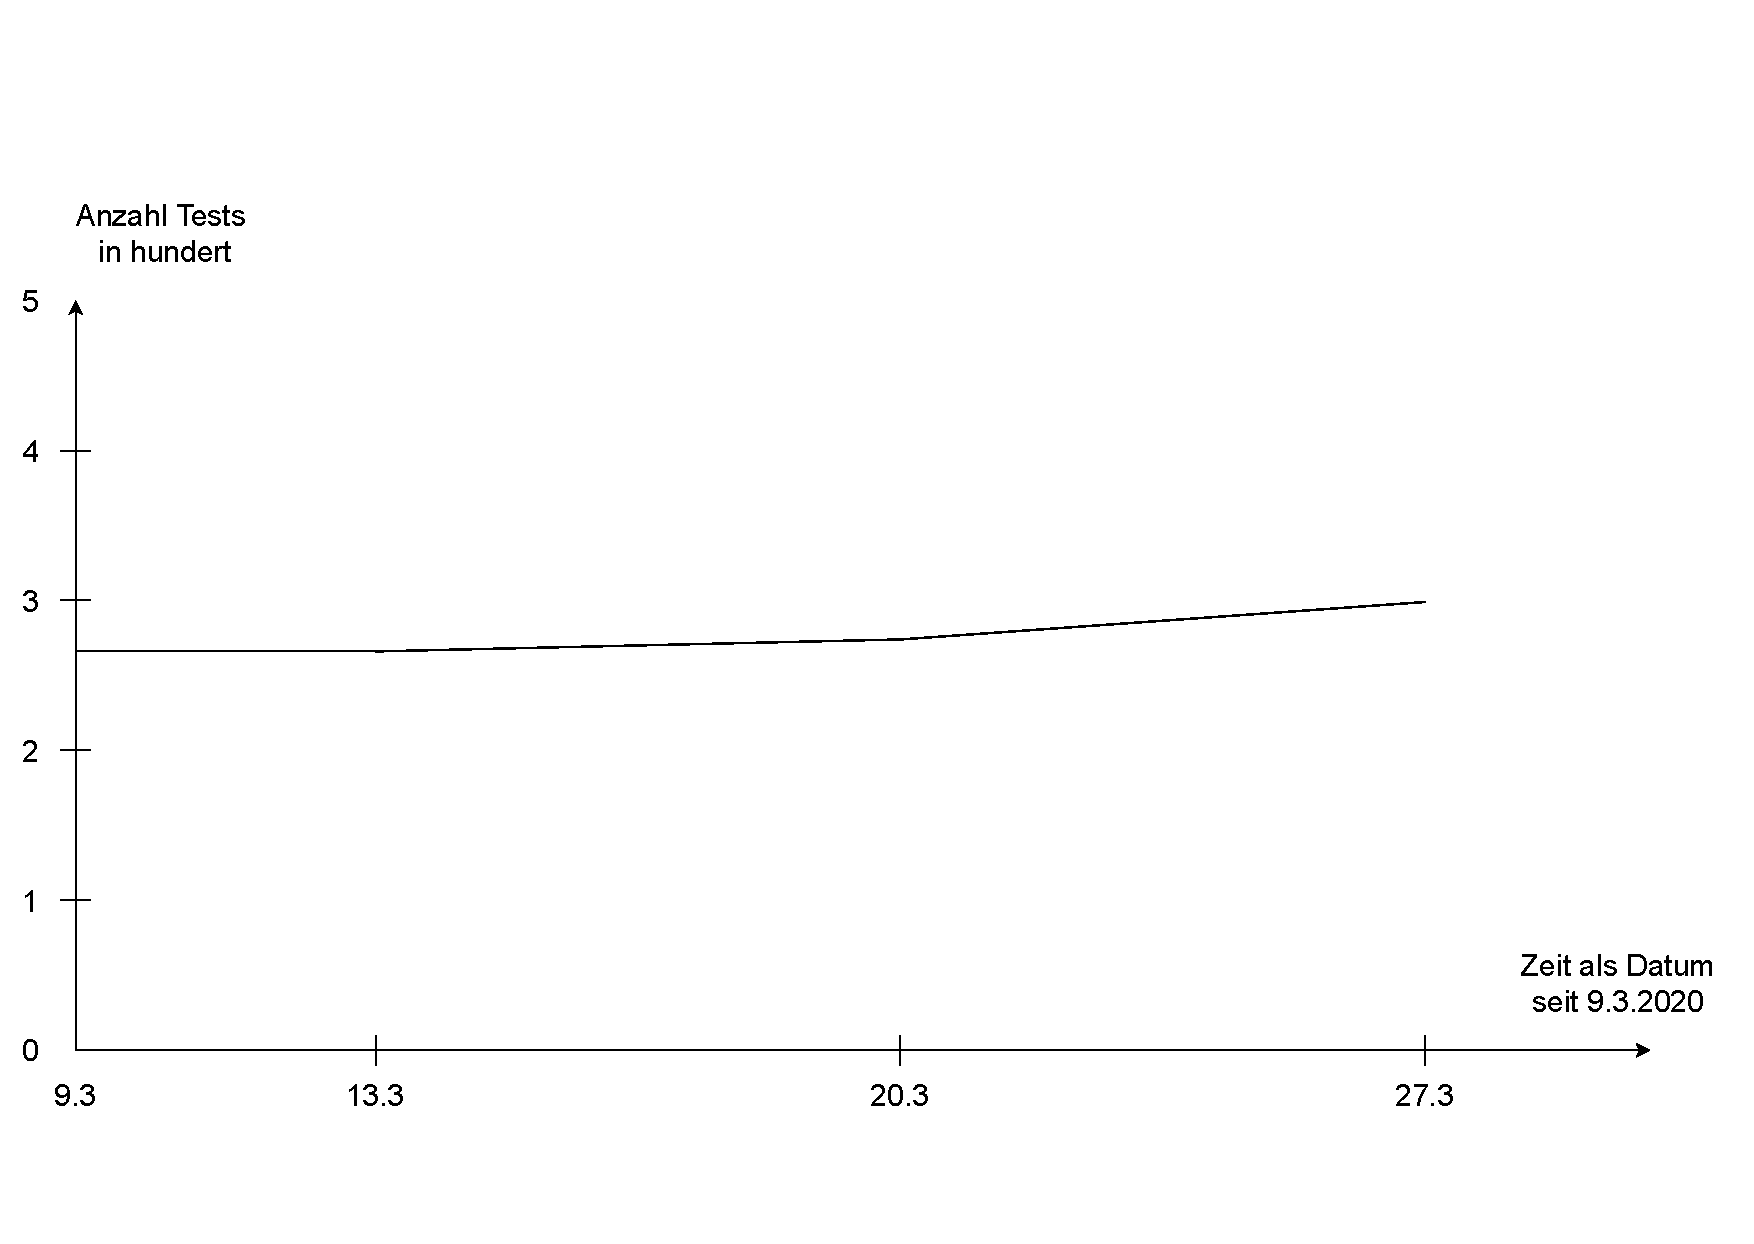
\includegraphics[width=\textwidth]{TestD} \newline
Da der Großteil des Codes bereits implementiert ist, sowie Integrationstests eher länger dafür aber weniger als Unittests sind, steigt auch die Anzahl der Tests nicht stark.
\clearpage
\subsection{Integrationstests}
\vspace{0.2cm}
Für das Automatisierte Testen des ganzen Systems haben wir ein Skript in Python benutzt, dieses beinhaltete diverse Szenarien und prüfte mit Positiv- als auch mit Negativtests. Neben diesem haben wir auch einiges "von Hand" getestet 
%Notiz an Jonas:
%Liste von Tests sodass wir bessere Tabellen erstellen können
\section{Umgesetzte Funktionale Anforderungen}

\begin{tabular}{|l|c|r|}
	\hline
	FA & Kurzbeschreibung & Implementiert? \\ \hline \hline
	FA1 & Client verbindet sich mit Server & Ja \\ \hline
	FA2 & Benutzer authentifiziert sich & Ja \\ \hline
	FA3 & Benutzer kann Aufgaben einreihen & Ja \\ \hline
	FA4 & Benutzer kann Parameter übergeben & Ja \\ \hline
	FA41 & Client speichert Parameter in Config & Ja \\ \hline
	FA42 & Benutzer kann Config übergeben & Ja \\ \hline
	FA43 & Benutzer kann Priorität festlegen & Ja \\ \hline
	FA44 & Benutzer kann min und max Cores festlegen & Ja \\ \hline
	FA45 & Benutzer kann min und max RAM festlegen & Ja \\ \hline
	FA46 & Benutzer kann Betriebssystem festlegen & Ja \\ \hline
	FA47 & Benutzer kann angeben ob Client blockiert & Ja \\ \hline
	FA48 & Benutzer übergibt Pfad zu Aufgabe & Ja \\ \hline
	FA49 & Es können Standardwerte benutzt werden & Ja \\ \hline
	FA5 & Benutzer kann Status von Aufgabe einsehen & Ja \\ \hline
	FA6 & Benutzer bekommt Email bei Abschluss & Ja \\ \hline
	FA7 & Server erstellt Backups & (Nein) \\ \hline
	FA8 & Benutzer kann Ausgabe anfordern & Ja \\ \hline
	FA9 & Benutzer kann Statistiken abfragen & Ja \\ \hline \hline
	OFA1 & Benutzer kann Restzeit einsehen & Nein \\ \hline
	OFA2 & Server stoppt lange Aufgaben & Nein \\ \hline
	OFA3 & Benutzer kann manuell Aufgaben stoppen & (Nein) \\ \hline
	OFA4 & Benutzer kann manuell Aufgaben sichern & (Nein) \\ \hline
	OFA5 & Benutzer kann Pausierbarkeit angeben & (Nein) \\ \hline
\end{tabular}
\newline \newline
Für Anforderungen mit einem (Nein) existiert zwar in manchen Teilen des Programms die Funktionalität dafür, die Funktion selber ist jedoch nicht umgesetzt oder nutzbar.
\section{Testen des Systems}
\subsection{Aufsetzen des Systems}
\vspace{0.2cm}
Welche Umgebung hatten wir, was haben wir im Endeffekt getestet (zb das aufsetzte Netz von Florian, eine Woche Testbetrieb)
\begin{itemize}[label={\textbullet}]
    \item Herunterladen des Programms unter\newline \texttt{https://github.com/balancedbanana/balancedbanana/releases}
    \item Einrichten der MySql Datenbank mit \newline
    \begin{mycode}
    cat balancedbanana.sql | sudo mysql
    \end{mycode}
    Die SQL Datei ist im Archiv unter \newline \texttt{share/balancedbanana/balancedbanana.sql} \newline
    zu finden.\newline
    Nun ist die Datenbank unter dem Schema balancedbanana installiert.
    In der MySQL-Konsole einen Datenbank Nutzer für balancedbanana anlegen mit folgenden MySQL-Befehlen:
    \begin{mycode}
    CREATE USER 'balancedbanana'@'localhost' IDENTIFIED BY 
    'balancedbanana';
    	
    GRANT ALL PRIVILEGES ON balancedbanana.* TO 'balancedbanana'@'localhost';
        
    FLUSH PRIVILEGES;
        
    exit
    \end{mycode}
    Das Passwort \texttt{balancedbanana} nach \texttt{IDENTIFIED BY} bei Bedarf anpassen und in \newline
    \texttt{share/balancedbanana/.bbs/appconfig.ini} \newline
    in Zeile \texttt{databasepassword} anpassen. \newline

\end{itemize}
\subsection{Konklusion}
Wie lief es, Leistung, entdeckte Bugs, etc.
\clearpage
\end{document}
